\documentclass[12pt,letter]{article}
\usepackage{mathptmx} % added for time new roman font
\usepackage[left=1in,right=1in,top=1in,bottom=1in]{geometry}
\usepackage[latin1]{inputenc}
\usepackage{amsmath}

\usepackage[textsize=tiny]{todonotes}

% defines all example enviorment
\usepackage[framemethod=tikz]{mdframed} % added for the box around examples
\newtheorem{ex}{Example}
\numberwithin{ex}{section} % allows for the use of example numbers that lign up with the section numbers
\newenvironment{example}{\begin{mdframed}[middlelinewidth=0.5mm]\begin{ex}\normalfont}{\end{ex}\end{mdframed}}

% defines all review enviorment
\usepackage[framemethod=tikz]{mdframed} % added for the box around examples
\newtheorem{re}{Review}
\numberwithin{re}{section} % allows for the use of example numbers that lign up with the section numbers
\newenvironment{review}{\begin{mdframed}[middlelinewidth=2mm,roundcorner=20pt]\begin{re}\normalfont}{\end{re}\end{mdframed}}

% defines the quotation enviorment 
\usepackage{xcolor}
\newcommand{\quotebox}[2]{\begin{center}\fcolorbox{white}{blue!15!gray!15}{\begin{minipage}{0.9\linewidth}\vspace{10pt}\center\begin{minipage}{0.8\linewidth}{\space\Huge``}{#1}{\Huge''}{\break\null\hfill} {\small #2}  \end{minipage}\medbreak\end{minipage}}\end{center}}

% defines the definition enviorment 
\newcommand{\definitionbox}[2]{\begin{center}\fcolorbox{white}{blue!15!gray!15}{\begin{minipage}{0.9\linewidth}\vspace{10pt}\center\begin{minipage}{0.8\linewidth} {{\textbf{Definition} - }{#1}: {#2}}\end{minipage}\medbreak\end{minipage}}\end{center}}

\usepackage{amsfonts}
\usepackage{amssymb}
\usepackage{graphicx}
\usepackage{float}
\usepackage{booktabs}
%\usepackage{parskip} % remove all the paragraph indents

\usepackage{setspace}
%\usepackage[colorlinks=true]{hyperref}
\usepackage{textcomp} 
\usepackage{multicol} 


%%%%%%%		define the symbols for positive directions		%%%%%%
\makeatletter													%%	
																%%					
\newcommand*\curveplus{% positive counterclockwise				%%
  \mathbin{\rotatebox[origin=c]{90}{$\m@th\curvearrowleft$}+}}	%%
																%%
\newcommand*\rightplus{% positive right							%%
  \mathpalette\@rightplus\relax}								%%
\newcommand*\@rightplus[1]{%									%%
  \mathbin{\vcenter{\hbox{$\m@th\overset{#1+}{\to}$}}}}			%%
																%%	
\newcommand*\upplus{% positive up								%%
  \mathbin{+\mathord\uparrow}}									%%
																%%			
\newcommand*\downplus{% positive down							%%		
  \mathbin{+\mathord\downarrow}}								%%
  																%%		
\newcommand*\downrightplus{% positive down and right			%%	
  \mathbin{+ \rotatebox[origin=c]{-30}{$\m@th\rightarrow$}}}	%%
\makeatother 													%%	
%%%%%%%%%%%%%%%%%%%%%%%%%%%%%%%%%%%%%%%%%%%%%%%%%%%%%%%%%%%%%%%%%%


\usepackage{mathtools}          %loads amsmath as well added for the piece wise function
\DeclarePairedDelimiter\Floor\lfloor\rfloor
\DeclarePairedDelimiter\Ceil\lceil\rceil

 
\newcounter{NumberInTable}
\newcommand{\LTNUM}{\stepcounter{NumberInTable}{(\theNumberInTable)}}

\newcommand{\Laplace}[1]{\ensuremath{\mathcal{L}{\left[#1\right]}}}
\newcommand{\InvLap}[1]{\ensuremath{\mathcal{L}^{-1}{\left[#1\right]}}}
\renewcommand{\textuparrow}{$\uparrow$}


\begin{document}



\setcounter{section}{5}	
\section{Vibration Control}

Throughout this text, we have studied various aspects related to analyzing and modeling vibrating systems. Therefore, it becomes prudent to look at methods for reducing or eliminating unwanted vibrations. However, before vibrations in a system can be effectively reduced they must be better understood in terms of their effects on the system under study. For this reason, this chapter first introduces the vibration Nomograph, this is then followed by vibration isolation, absorption, and active suppression.  

\subsection{Vibration Nomograph}

There exist various methods and standards for measuring and describing acceptable levels of vibrations in systems, these include ISO/AWI 2631 for the evaluation of human exposure to whole-body vibrations and ISO 4866 for the measurement and effects of vibrations on structures. A common way to present the acceptable limit of vibration is in a vibration nomograph.  A vibration nomograph is a simplified way to express the acceptable limits on a system while considering the displacement, velocity, acceleration, and frequency of a system. A typical nomograph with various limits is presented in figure \ref{fig:Vibration_nomograph}. 

A vibration nomograph is a logarithmic plot that allows us to easily express the relationships between displacement, velocity, acceleration, and frequency of a system. The vibration nomograph presented in figure \ref{fig:Vibration_nomograph} considers an undamped 1-DOF system with constant amplitude ($A$) experiencing harmonic motion that can be modeled as:
\begin{equation}
    x(t) = A \sin(\omega t)
    \label{eq:displacement}
\end{equation}
Therefore, the velocity and acceleration terms can be found by taking the derivatives of the displacement expression to yield:
\begin{equation}
    \dot{x}(t) = A \omega \cos(\omega t)
\end{equation}
and:
\begin{equation}
    \ddot{x}(t) = -A\omega^2 \sin(\omega t)
    \label{eq:acceleration}
\end{equation}
These equations are converted from a circular frequency in rad/sec to a linear frequency ($f$) in Hz, such that $\omega = 2\pi f$. Therefore, equations \ref{eq:displacement}-\ref{eq:acceleration} become:
\begin{equation}
    x(t) = A \sin(\omega t)
\end{equation}
\begin{equation}
    v(t) =  \dot{x}(t) = 2\pi f A \cos(\omega t)
\end{equation}
\begin{equation}
    a(t) =  \ddot{x}(t) = -4\pi^2 f^2 A \sin(\omega t)
\end{equation}
Thereafter, the maximum values for velocity $v_\text{max}$ and acceleration $a_\text{max}$ are related to amplitude through:
\begin{equation}
    v_\text{max} = 2\pi f A 
    \label{eq:v_max}
\end{equation}
\begin{equation}
    a_\text{max} = -4\pi^2 f^2 A = -2 \pi f v_\text{max}
    \label{eq:a_max}
\end{equation}
by taking the natural log of both side of equation \ref{eq:v_max} we obtain: 
\begin{equation}
    \ln v_\text{max} = \ln(2\pi f) + \ln A
    \label{eq:ln_v_max} 
\end{equation}
doing the same for equation \ref{eq:a_max} leads to:
\begin{equation}
     \ln a_\text{max} = - \ln(2\pi f) - \ln v_\text{max}
    \label{eq:ln_v_max_2} 
\end{equation}
It can be seen that both of these expressions are linear. 

The nomograph sets the $x-$axis as frequency in Hz and the $x-$axis as velocity in mm/s. Equation \ref{eq:ln_v_max} tells us that For a constant amplitude of displacement ($A$), $\ln v_\text{max}$ is linearly proportional to $\ln (2 \pi f)$, at a rate of $2 \pi$. As the $x-$axis in a nomograph is frequency, measured in Hz and thereby accounting for the $2 \pi$, $\ln (2 \pi f)$ is a straight line with a positive slope of 1 with respect the frequency axis (i.e. $x-$axis). Therefore, a line on the nomograph that represents a constant displacement is at a 45$^\circ$ angle from the $x$-axis. 


For a constant value of velocity, ($v_\text{max}$), equation \ref{eq:ln_v_max_2} shows that acceleration ($\ln a_\text{max}$) is linearly proportional to $-\ln (2 \pi f)$, at a rate of $2 \pi$. Again, as the $x-$axis in a nomograph is frequency, measured in Hz, acceleration is represented by a straight line that varies with $- \ln(2\pi f)$, therefore, $\ln a_\text{max}$ is a straight line with the slope of -1. This is also represented by a line of constant acceleration set at a -45$^\circ$ angle from the $x$-axis. These equations are expressed in the vibration nomograph plot of figure \ref{fig:Vibration_nomograph} where each point on the plot represents a specific sinusoidal (harmonic) vibration for a 1-DOF system.  

\begin{figure}[H]
    \centering
    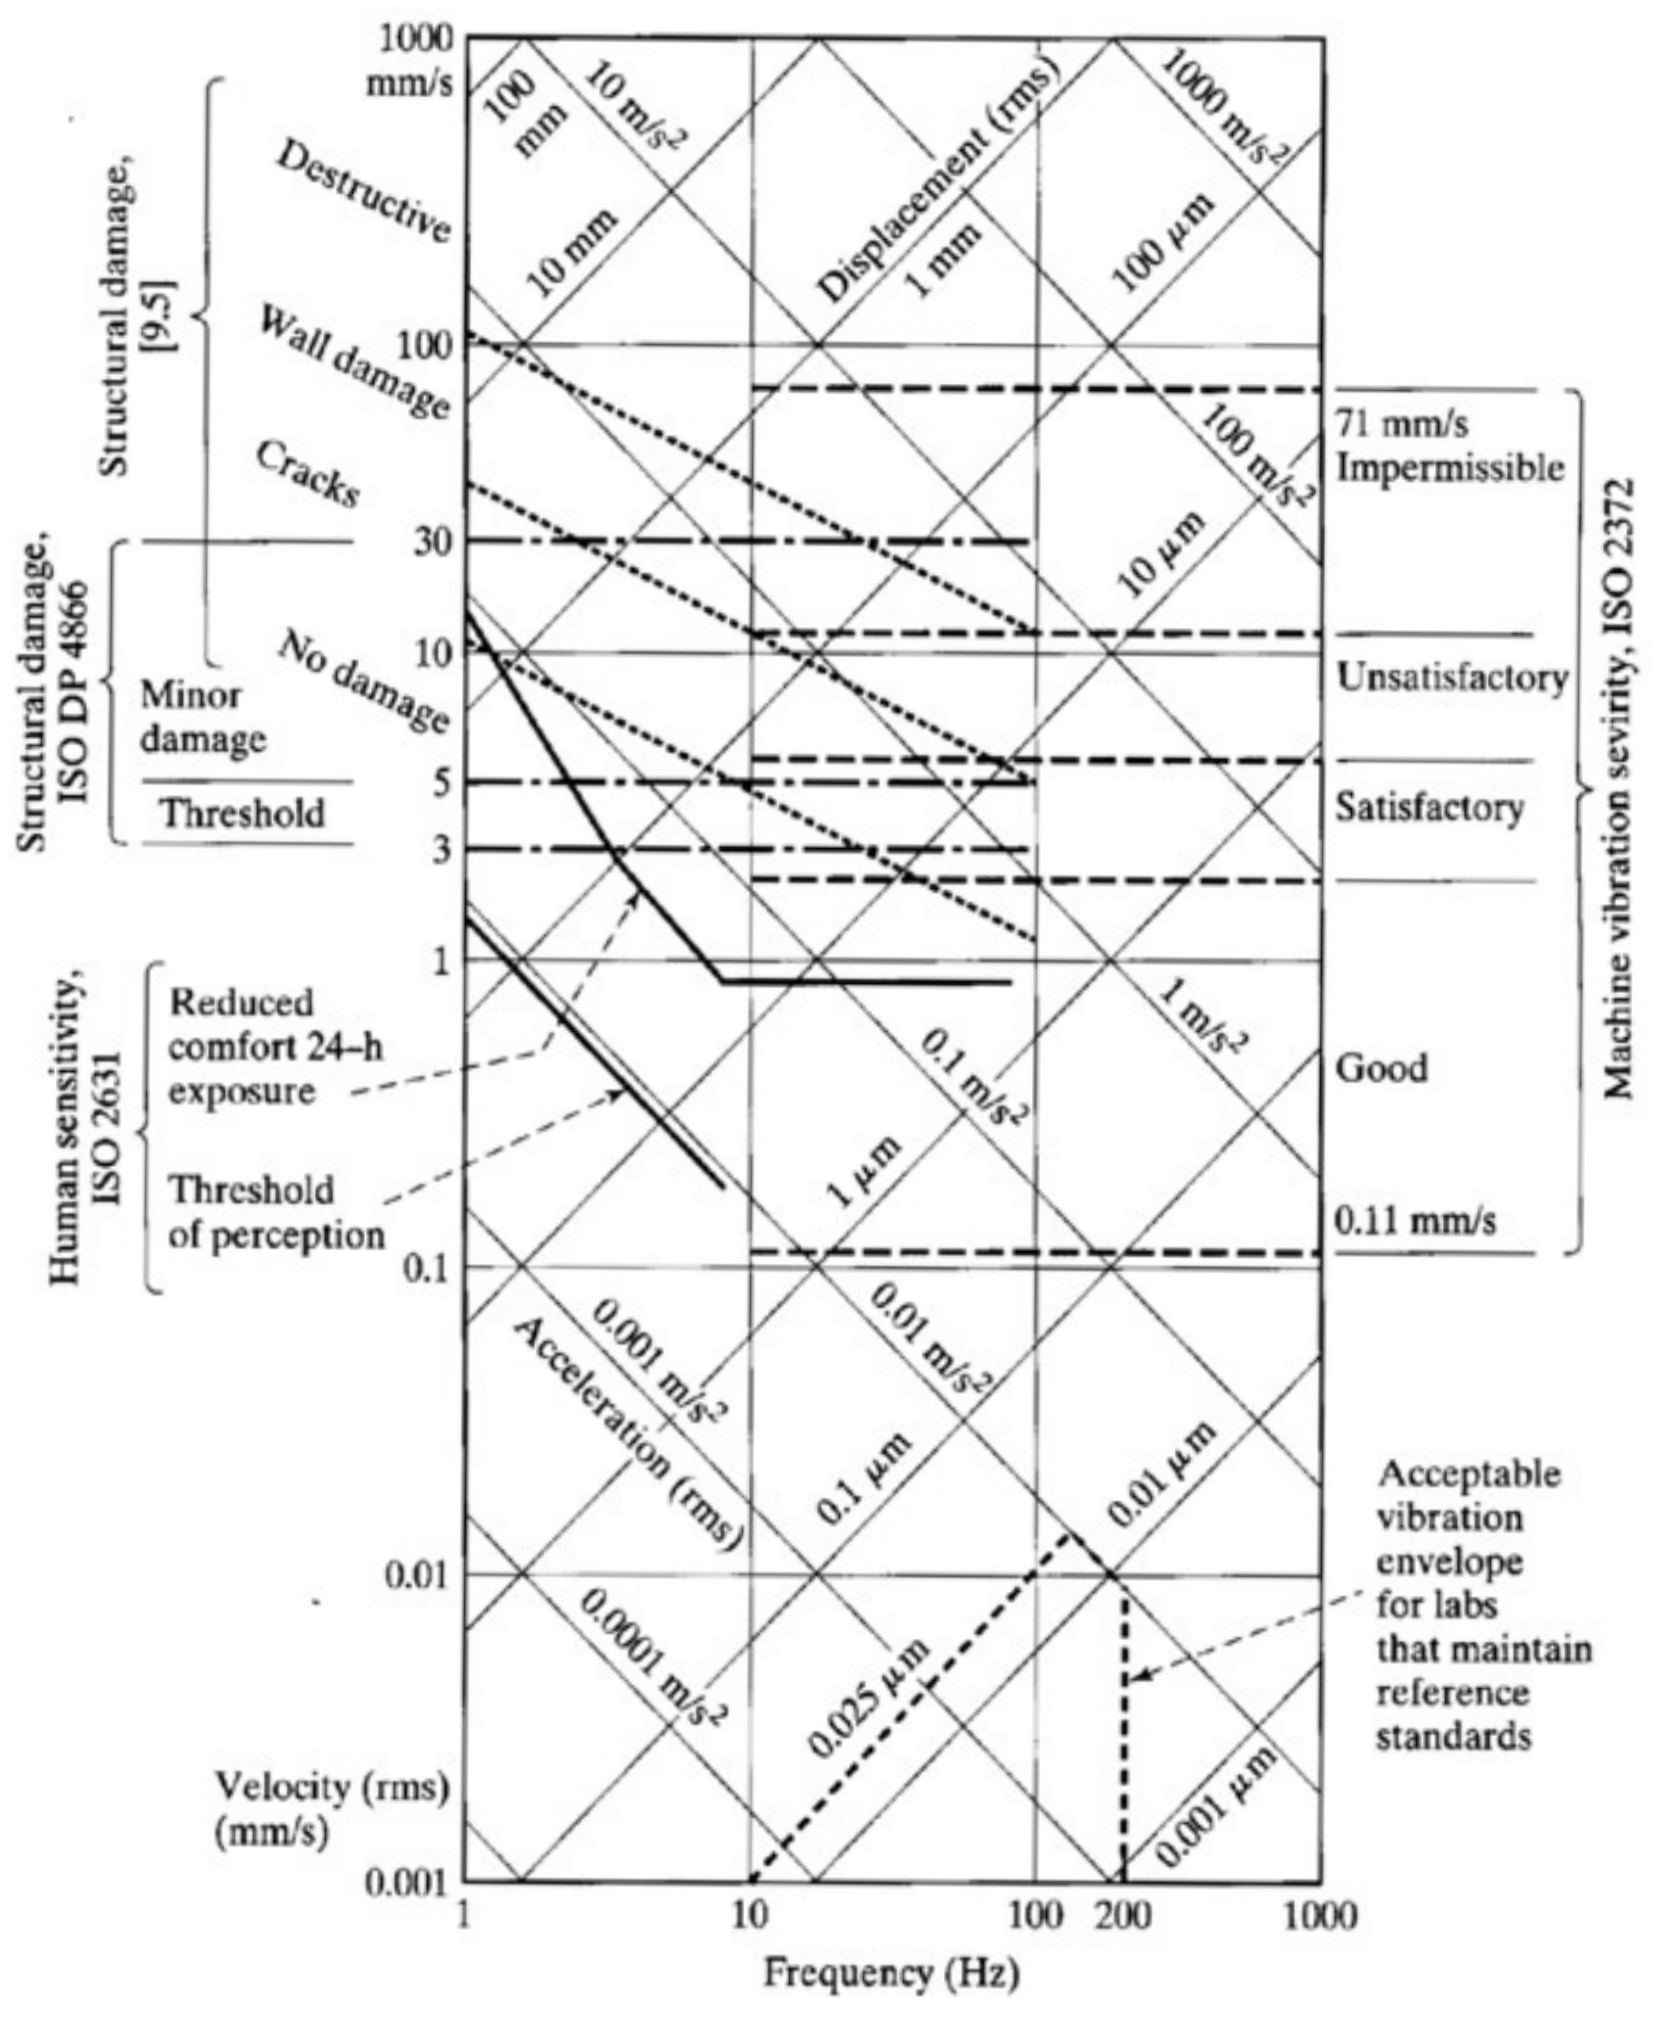
\includegraphics[width=4.5in]{../Figures/Vibration_nomograph.png}
    \caption{Vibration nomograph showing the acceptable limits of vibration for various applications.}
    \label{fig:Vibration_nomograph}
\end{figure}


\subsection{Vibration Isolation}



\subsection{Vibration Absorption}

Vibration absorbers, also termed dynamic vibration absorber, are a class of mechanical devices that seek to reduce unwanted vibrations in a system. In contrast to a traditional dash-pot style damper, these systems seek to ``redirect'' the vibrations from the system to another mass connected to the system. In this way the main system is protected form the bandwidth of vibrations that the vibration absorbers is tuned for. As the vibration absorbers must be tuned for the system, it is generally limited to devices that operate at a fixed frequency like industrial equipment or cables suspended in the air and subjected to wind loading. Figure~\ref{fig:vibration_absorbers} presents a Stockbridge and a Dogbone damper designed to remove certain bandwidths of excitation form wind-excited cables.

\begin{figure}[H]
    \centering
    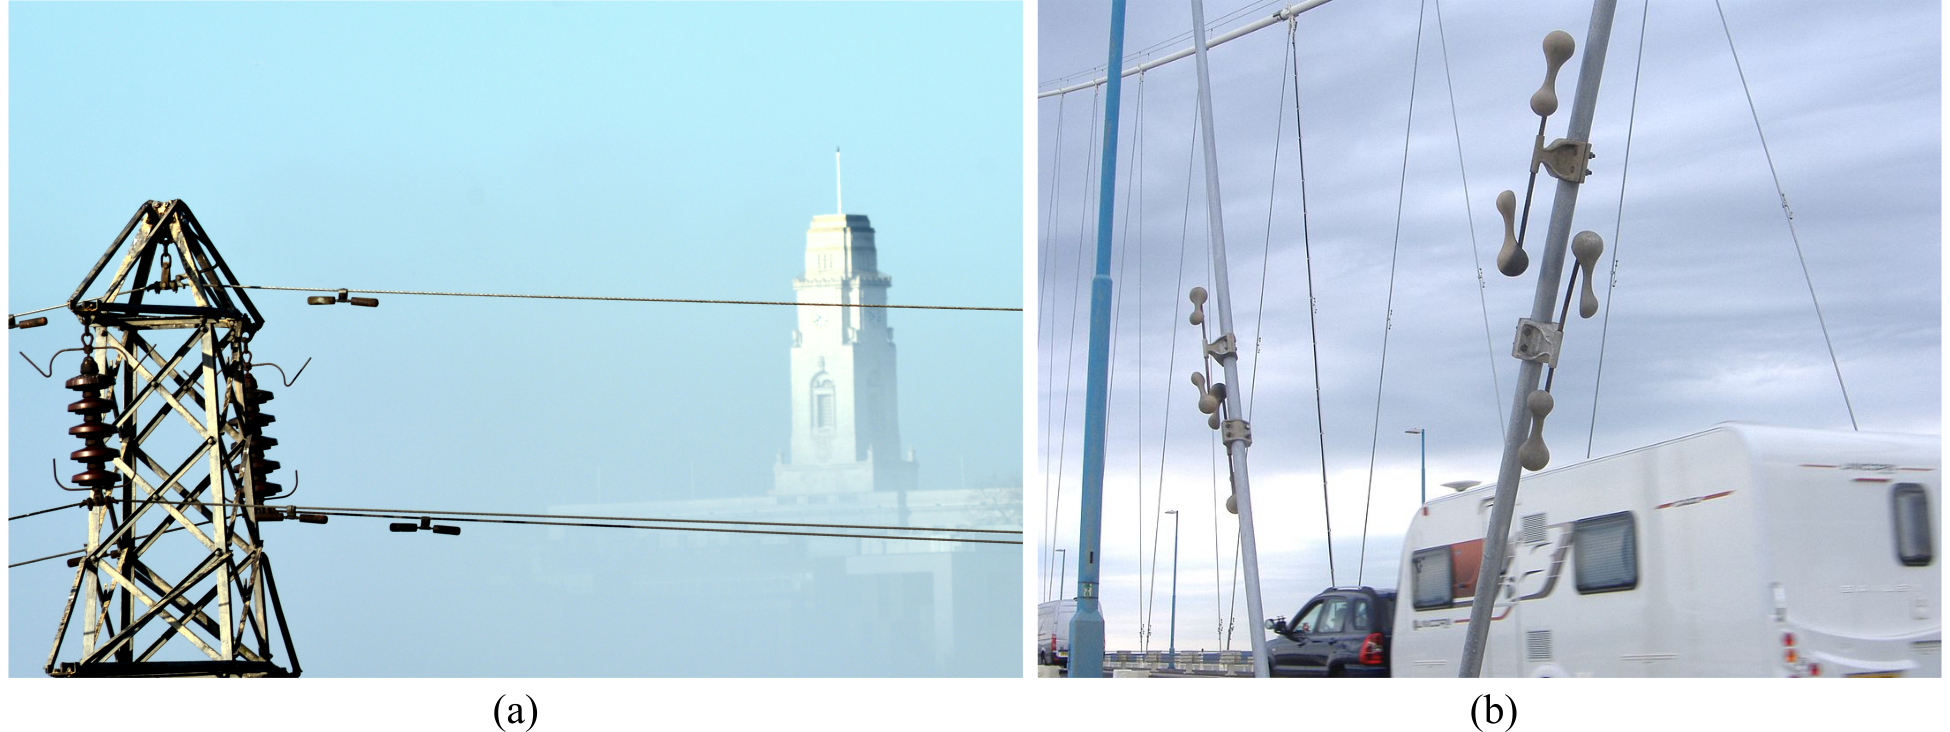
\includegraphics[width=6.5in]{../Figures/vibration_absorbers.png}
    \caption{Vibration absorbers deployed on wind excited cables showing: (a) a Stockbridge damper on a high-power transmission line\protect\footnotemark[1], and; (b) a dogbone damper on a suspender cable of a suspension bridge\protect\footnotemark[2].}
    \label{fig:vibration_absorbers}
\end{figure}
\footnotetext[1]{``Stockbridge dampers installed on high voltage power lines'' by Badics CC BY-SA 3.0}  
\footnotetext[2]{``Dogbone dampers on the road-support cables of the Severn Bridge'' by Bassaar  CC BY-SA 4.0}  

Vibration absorbers are most often designed to shift the resonance frequency of the first mode of the system away from the expected excitation frequency. This is done by adding an additional degree-of-freedom in the form of a mass (the vibration absorber) connected to system with a spring to alter the natural frequency of the combined system away from the original excitation frequency. Dashpots may also be added in parallel to the spring element if additional energy dissipation in needed beyond that provided by the original system. 

\begin{figure}[H]
    \centering
    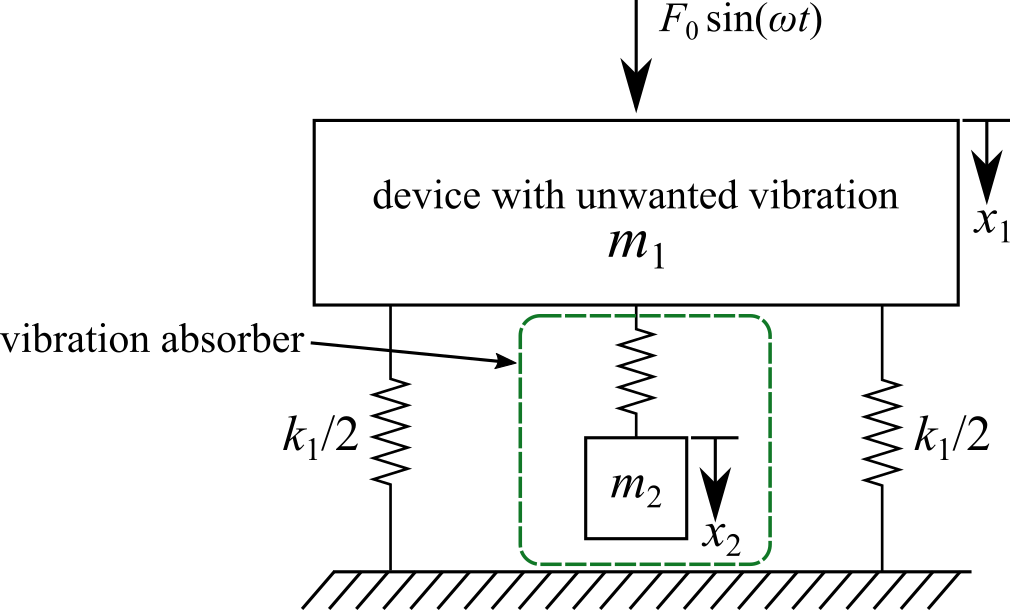
\includegraphics[]{../Figures/vibration_absorber_spring_mass.png}
    \caption{A vibration absorber ($m_2$) for mitigating unwanted dynamics in a device ($m_1$).}
    \label{fig:vibration_absorber_spring_mass}
\end{figure}

The tuning of a 2-DOF system can be done by setting the displacement of the mass to be controlled to zero and solving for the mass and stiffness of vibration absorber. Consider the system presented in figure~\ref{fig:vibration_absorber_spring_mass}, here $m_1$ and $k_1$ are the mass and stiffness of the system while $m_2$ and $k_2$ are the mass and stiffness of the vibration absorber. A good assumption to make when designing a vibration absorber is that the mass of the absorber should be between 1\% and 5\% of the mass of the system to be damped. Therefore, for this case let $m_1$ = 20 kg, $m_2$ = 1 kg, and $k_1$ = 20 kN. Assuming a sinusoidal input where $F_0 = 1$ kN, the equations of motion are:
\begin{equation}
m_1\ddot{x_1} + k_1 x_1 + k_2(x_1-x_2)  = F_0 \sin (\omega t)
\end{equation}
\begin{equation}
m_2\ddot{x_2} + k_2(x_2-x_1) = 0
\end{equation}
Assuming the temporal solution is of a harmonic form, the following is true:
\begin{equation}
x_i(t) = X_i \sin (\omega t ), \; \; i=1,2
\end{equation}
using the transfer function approach and assuming no initial conditions, the following steady state solution can be obtained for $m_1$ and $m_2$:
\begin{equation}
X_1 = \frac{(k_2 - m_2 \omega^2)F_0}{(k_1+k_2-m_1 \omega^2)(k_2-m_2 \omega^2) -k_2^2}
\label{eq:X1_displacement}
\end{equation}
\begin{equation}
X_2 = \frac{k_2 F_0}{(k_1+k_2-m_1 \omega^2)(k_2-m_2 \omega^2) -k_2^2}
\label{eq:X2_displacement}
\end{equation}
Next, the natural frequency of $m_1$ ($\omega_1$) can be solved for as $\omega_1=\sqrt{k_1 / m_1}$. In order to eliminate movement for $m_1$ at a given driving frequency $\omega$, the numerator of equation~\ref{eq:X1_displacement} should be set to zero. Note that setting $F_0$ is a trivial solution and provides no real benefit to the system. Therefore:
\begin{equation}
k_2 = m_2 \omega^2
\end{equation}
note that this will force the frequency of the tuned vibration absorber to match that of the system, therefore $\omega_1 = \omega_2 = \sqrt{k_2 / m_2}$. Next, normalizing the input force $F_0$ by the stiffness of the main system $k_1$ yields:
\begin{equation}
\delta_{\text{st}} = \frac{F_0}{k_1}
\end{equation}
using this term, equations~\ref{eq:X1_displacement} and \ref{eq:X2_displacement} can be rearranged as:
\begin{equation}
\frac{X_1}{\delta_{\text{st}}} = \frac{1 - \big(\frac{\omega}{\omega_2} \big)^2 }{\Big[1 + \frac{k_2}{k_1} - \big(\frac{\omega}{\omega_1} \big)^2 \Big] \Big[ 1- \big(\frac{\omega}{\omega_2} \big)^2 \Big] -\frac{k_2}{k_1}}
\label{eq:X1_norm_displacement}
\end{equation}
\begin{equation}
\frac{X_2}{\delta_{\text{st}}} = \frac{1}{\Big[1 + \frac{k_2}{k_1} - \big(\frac{\omega}{\omega_1} \big)^2 \Big] \Big[ 1- \big(\frac{\omega}{\omega_2} \big)^2 \Big] -\frac{k_2}{k_1}}
\label{eq:X2_norm_displacement}
\end{equation}
Figure~\ref{fig:vibration_absorber_undamped_results} reports the normalized displacement of the system over a frequency range for system with and without a vibration absorber. Note that at $\omega=1$ the original system is in resonance while the system with the vibration absorber has no displacement. However, no system is without compromise. From equation~\ref{eq:X2_norm_displacement} it can be seen that at $\omega = \omega_1 = \omega_2$ the second mass needs a displacement equal to:
\begin{equation}
X_2 = -\frac{k_1}{k_2}\delta_{\text{st}} = -\frac{F_0}{k_2}
\end{equation}
or 1 m using the given parameters. Therefore, the mass and stiffness values of the vibration absorber should be selected based the the allowable travel of the absorber (i.e. $X_2$), among other factors. Moreover, from this equation it can be seen the force exerted by the second mass operates in the direction opposite the original force ($-F_0 - k_2 X_2$), thereby canceling it. Lastly, note that the addition of the vibration absorber creates two resonate frequencies of the system, termed $\Omega_1$ and $\Omega_2$. These  resonate frequencies represent roots of the system and care should be taken to limit the time the system spends at these frequencies (i.e. on startup). The locations of these roots can be solved for analytically by setting the denominators of equation \ref{eq:X1_norm_displacement} to zero.



\begin{figure}[H]
    \centering
    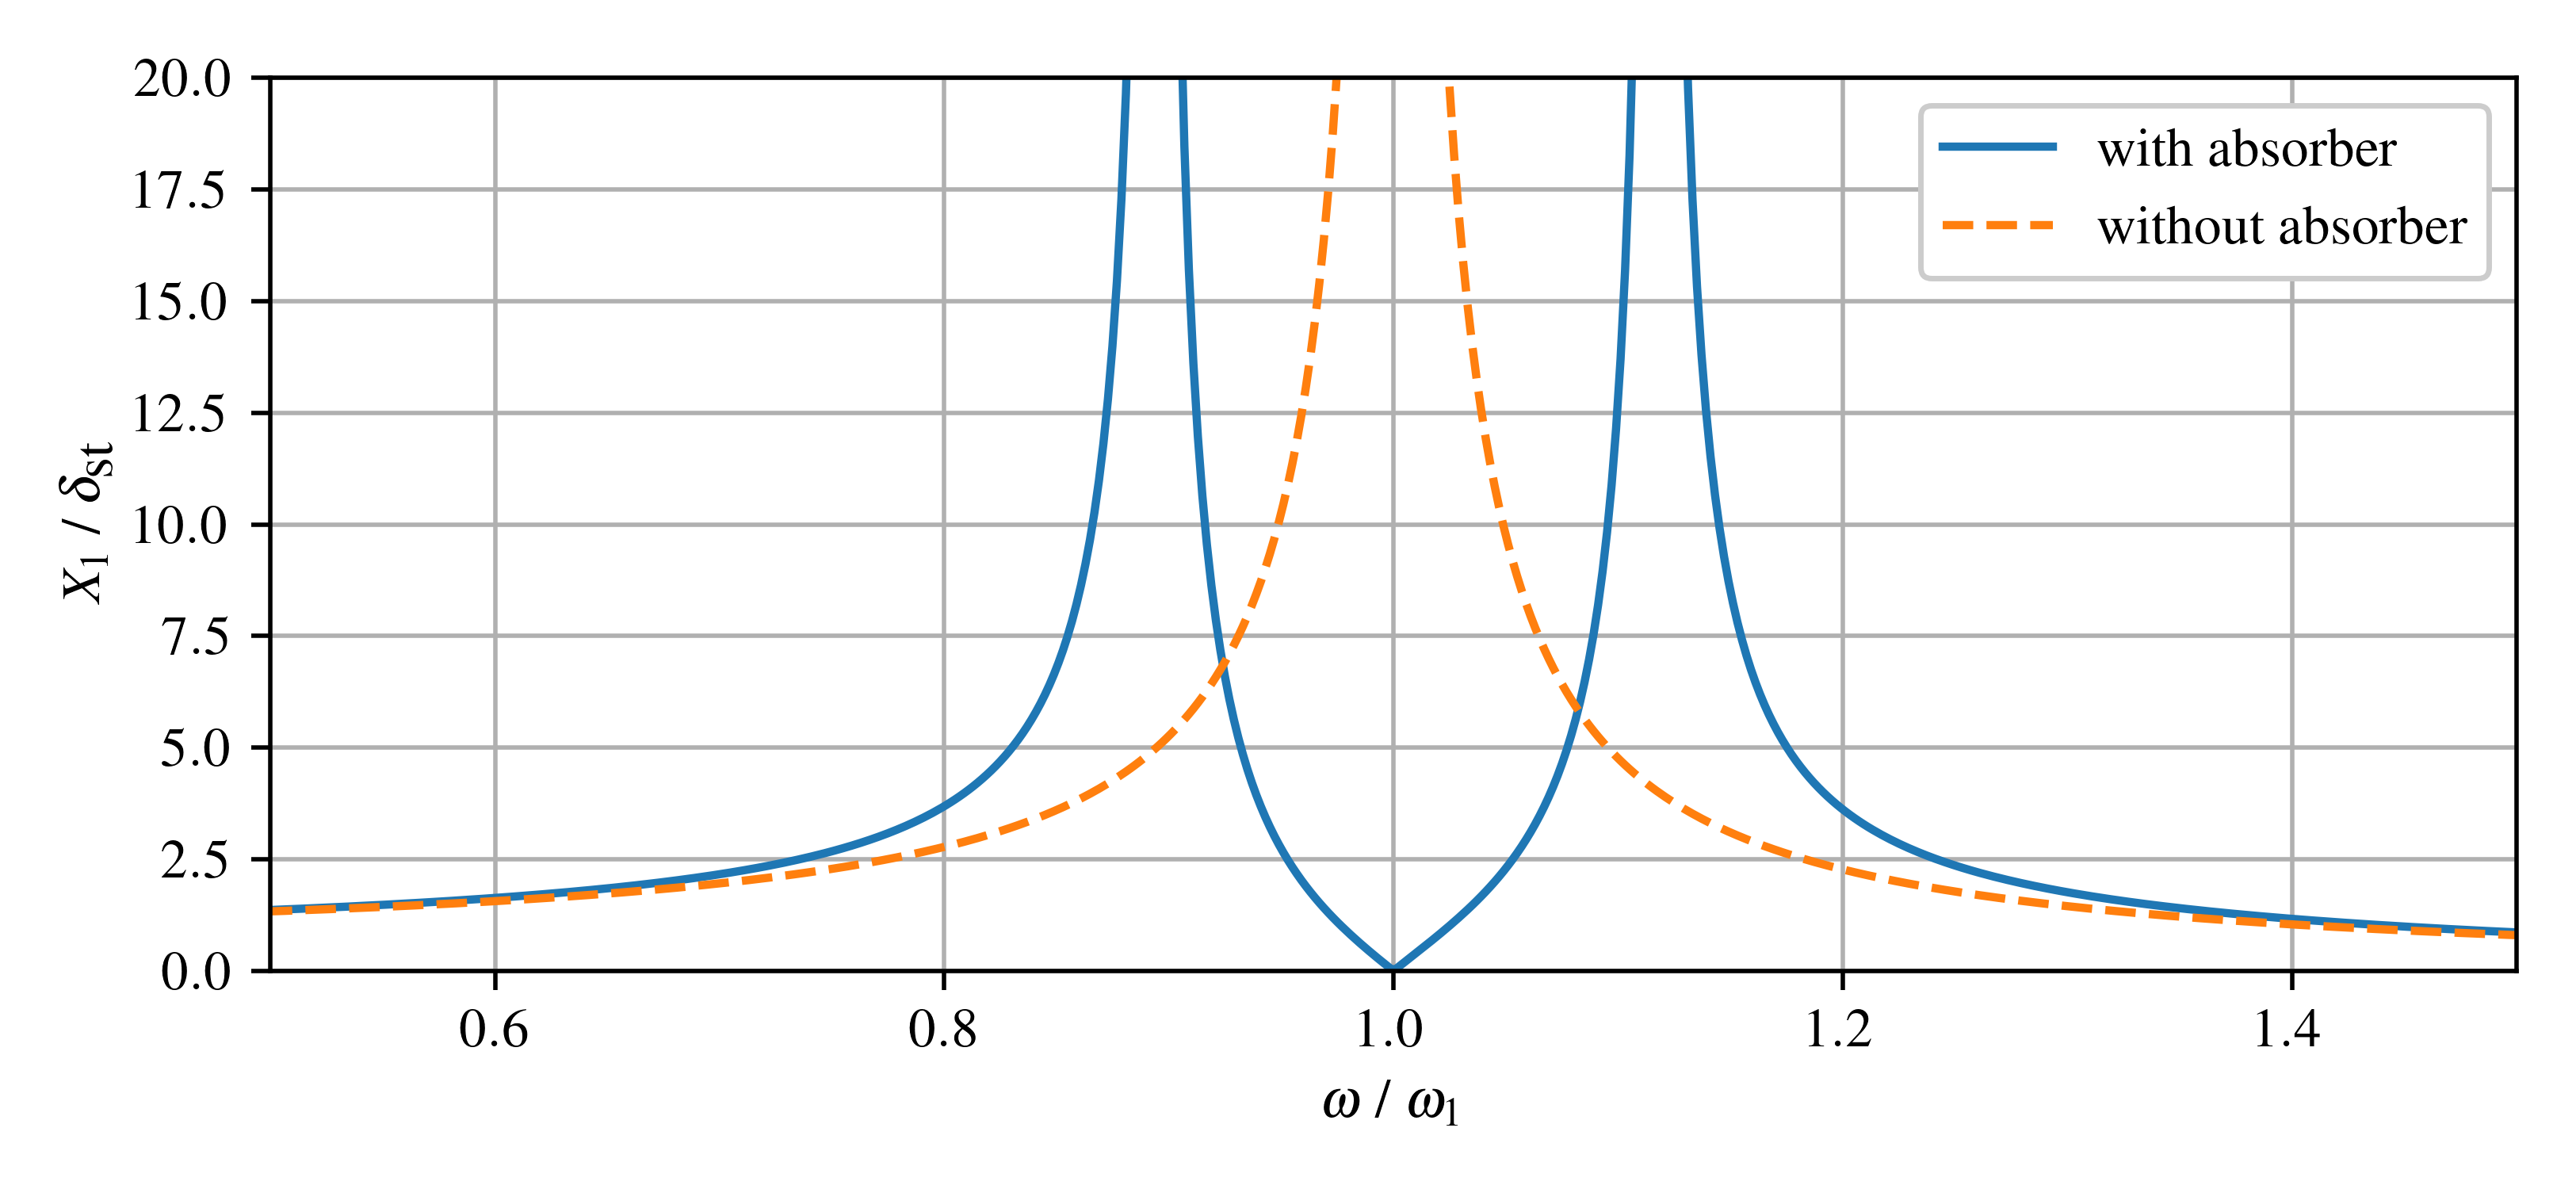
\includegraphics[width=6.5in]{../Figures/vibration_absorber_undamped_results.png}
    \caption{Frequency response of the undamped system with and without the vibration absorber.}
    \label{fig:vibration_absorber_undamped_results}
\end{figure}







\subsection{Active Vibration Suppression}

Active vibration control add energy to the system in order to mitigate the vibrations in the system. As depicted in figure \ref{fig:active_vibration_control_FBD}(a), an active vibration control system requires a sensor to acquire data from the system, control hardware and algorithms to processes this data, and an actuator to exert a physical control on the system. These system together are called a feedback loop, as a movement in the mass results in a control force $(f_u)$ being exerted on the system. This control force is diagrammed in figure \ref{fig:active_vibration_control_FBD}(b). 

\begin{figure}[H]
    \centering
    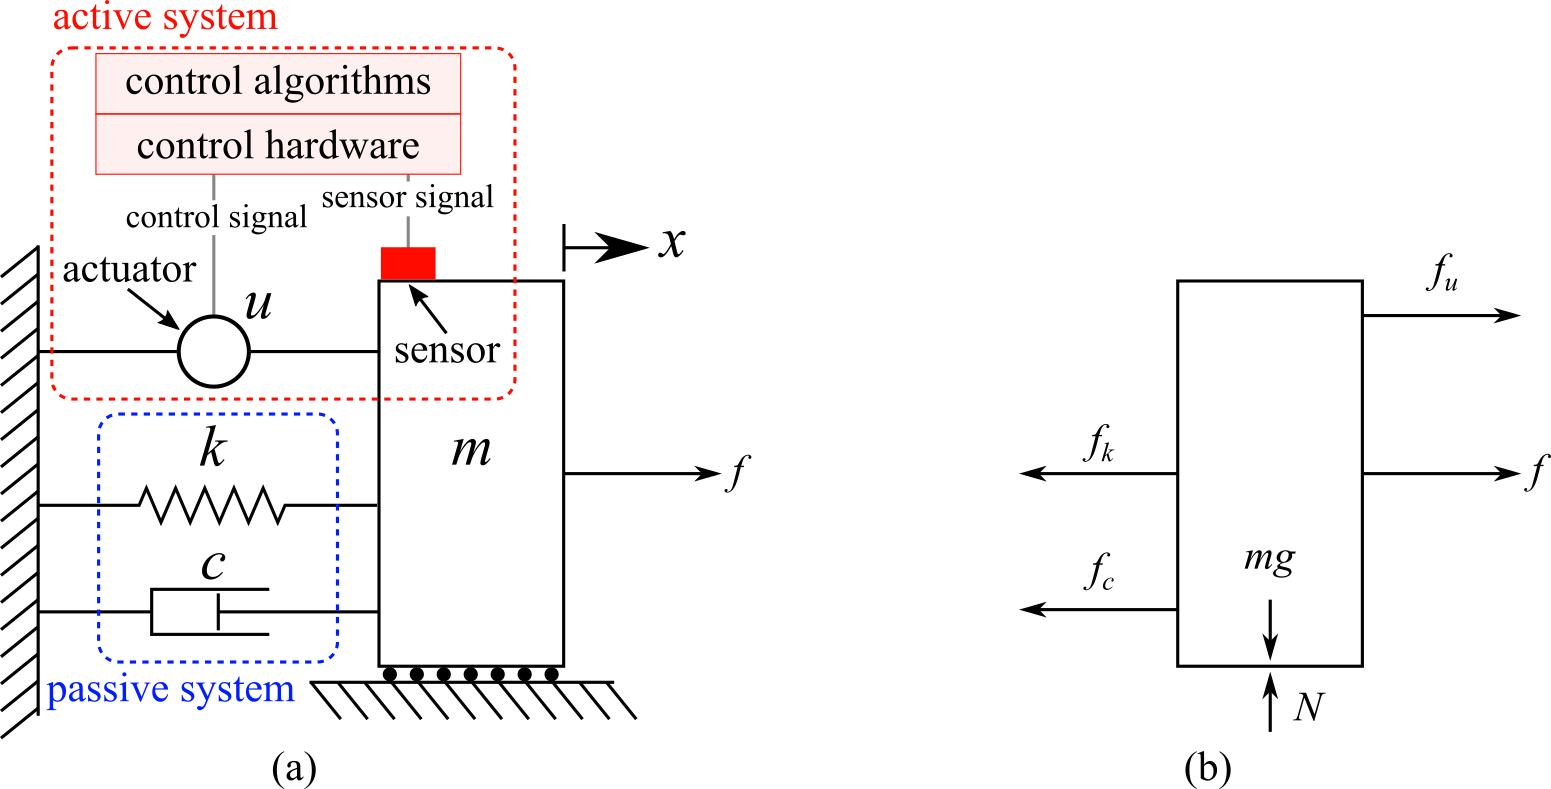
\includegraphics[width=5in]{../Figures/active_vibration_control_FBD.png}
    \caption{Active vibration control system showing: (a) the system with a feed-back loop that takes a signal from the sensor, converts it to a control signal, and drives the actuator; and (b) the free body diagram.}
    \label{fig:active_vibration_control_FBD}
\end{figure}

Adding the control force to the EOM for the 1-DOF system presented in figure \ref{fig:active_vibration_control_FBD} results in:
\begin{equation}
m \ddot{x} + c \dot{x} + kx = F(t) = f + f_u
\end{equation}
A common method for providing control for vibration suppression is called position derivative control or PD-control. PD-control measures the position and velocity of the mass and uses these to compute the control force needed to mitigate the vibration to an acceptable level. A simple way to code a PD-controller is to provide a control force proportional to the displacement velocity (derivative of displacement) of the mass such that:
\begin{equation}
f_u = -g_1x - g_2 \ddot{x}
\end{equation}
where $g_1$ and $g_2$ are the proportional gains of the systems. The control gains can be constants determined by the designer or variables updated through time by an algorithm. Here we will consider the gains to be constant, therefore, the EOM for the closed-loop system in figure \ref{fig:active_vibration_control_FBD} becomes:
\begin{equation}
m \ddot{x} + (c + g_2) \dot{x} + (k + g_1)x = F(t) = f 
\end{equation}
This formulation lets $g_1$ act as additional damping while $g_2$ acts as additional damping. This closed-loop EOM can be used to solve for the effective natural frequency of the system, given by:
\begin{equation}
\omega_n = \sqrt{\frac{k+g_p}{m}}
\end{equation}
and the effective damping ratio of the system
\begin{equation}
\zeta = \frac{c+g_2}{2\sqrt{m(k+g_1)}}
\end{equation}



























			\noindent
			

	\pagebreak
	\renewcommand{\thepage}{}
	\renewcommand\refname{References Cited}
	\pagestyle{plain}
	\bibliographystyle{unsrtDOI}
	\bibliography{Chapter_6_vibration_control}
	
\end{document}














